\documentclass[a4paper, 11pt]{article}
\usepackage{multicol}
\usepackage{tabularx}
\usepackage{enumitem}
\usepackage[a4paper, margin=1.8cm]{geometry}
\usepackage{listings}
\usepackage{amssymb}
\usepackage{gvv}
\usepackage{gvv-book}
\usepackage{amsmath}
\usepackage{setspace}
\usepackage{caption}

\graphicspath{ {./figs/} }
\begin{document}
\begin{center}
    \huge{CS: COMPUTER SCIENCE AND INFORMATION TECHNOLOGY}\\
    \large{EE25BTECH11041 - Naman Kumar}
\end{center}
 \begin{enumerate}
     \item A binary operation $\bigoplus$ on a set of integers is defined as $x\bigoplus y=x^2+y^2$ Which one of the following statements is TRUE about $\bigoplus$ ?
    \begin{enumerate}
        \begin{multicols}{2}
            \item Commutative but not associative
            \item Both commutative and associative 
            \item Associative but not commutative 
            \item Neither commutative nor associative 
        \end{multicols}
    \end{enumerate}

    \hfill (GATE CS 2013)
    
    \item Suppose p is the number of cars per minute passing through a certain road junction between 5 PM and 6 PM, and p has a Poisson distribution with mean 3. What is the probability of observing fewer than 3 cars during any given minute in this interval?
    \begin{enumerate}
        \begin{multicols}{4}
            \item $8/(2e^3)$
            \item $9/(2e^3)$
            \item $17/(2e^3)$
            \item $26/(2e^3)$
        \end{multicols}
    \end{enumerate}
    
    \hfill (GATE CS 2013)
    
    \item Which one of the following does NOT equal\myvec{1 & x & x^2\\1 & y & y^2\\1 & z & z^2}
    \begin{enumerate}
        \begin{multicols}{2}
    \item 
    \[
    \mydet{
        1 & x(x+1) & x+1\\
        1 & y(y+1) & y+1\\
        1 & z(z+1) & z+1
    }
    \]

    \item 
    \[
    \mydet{
        1 & x+1 & x^2+1\\
        1 & y+1 & y^2+1\\
        1 & z+1 & z^2+1
    }
    \]

    \item 
    \[
    \mydet{
        0 & x-y & x^2-y^2\\
        0 & y-z & y^2-z^2\\
        1 & z & z^2
    }
    \]

    \item 
    \[
    \mydet{
        2 & x+y & x^2+y^2\\
        2 & y+z & y^2+x^2\\
        1 & z & z^2
    }
    \]

        \end{multicols}
    \end{enumerate}

    \hfill (GATE CS 2013)
    
    \item The smallest integer that can be represented by an 8-bit number in 2’s complement form is 
    \begin{enumerate}
        \begin{multicols}{4}
            \item -256
            \item -128
            \item -127
            \item 0
        \end{multicols}
    \end{enumerate}

    \hfill (GATE CS 2013)
    
    \item In the following truth table, V = 1 if and only if the input is valid. \\
    \begin{table}[H]
    \centering
    \begin{tabular}{|c|c|c|c||c|c|c|}
    \hline
    \multicolumn{4}{|c||}{\textbf{Inputs}} & \multicolumn{3}{c|}{\textbf{Outputs}} \\ \hline
    $D_0$ & $D_1$ & $D_2$ & $D_3$ & $X_0$ & $X_1$ & $V$ \\ \hline
    0 & 0 & 0 & 0 & x & x & 0 \\ \hline
    1 & 0 & 0 & 0 & 0 & 0 & 1 \\ \hline
    x & 1 & 0 & 0 & 0 & 1 & 1 \\ \hline
    x & x & 1 & 0 & 1 & 0 & 1 \\ \hline
    x & x & x & 1 & 1 & 1 & 1 \\ \hline
    \end{tabular}
    \end{table}
    What function does the truth table represent? 
    \begin{enumerate}
        \begin{multicols}{2}
            \item Priority encoder
            \item Decoder
            \item Multiplexer
            \item Demultiplexer
        \end{multicols}
    \end{enumerate}
    
    \hfill (GATE CS 2013)
    
    \item Which one of the following is the tightest upper bound that represents the number of swaps required to sort n numbers using selection sort?  
    \begin{enumerate}
        \begin{multicols}{4}
            \item $O(\log n)$
            \item $O(n)$
            \item $O(n \log n)$
            \item $O(n^2)$
        \end{multicols}
    \end{enumerate}
    
    \hfill (GATE CS 2013)
    
    \item Which one of the following is the tightest upper bound that represents the time complexity of inserting an object into a binary search tree of n nodes? 
    \begin{enumerate}
        \begin{multicols}{4}
            \item $O(1)$
            \item $O(\log n)$
            \item $O(n)$
            \item $O(n \log n)$
        \end{multicols}
    \end{enumerate}
    
    \hfill (GATE CS 2013)
    
    \item  Consider the languages $L_1 =\phi $ and $ L_2 ={a }.$ Which one of the following represents $L_1L_2^*\bigcup L_1* $ ? 
    \begin{enumerate}
        \begin{multicols}{4}
            \item $\{c\}$
            \item $\phi$
            \item $a^*$
            \item $\{\epsilon,a\}$
        \end{multicols}
    \end{enumerate}
    \hfill (GATE CS 2013)
    \item What is the maximum number of reduce moves that can be taken by a bottom-up parser for a grammar with no epsilon- and unit-production (i.e., of type A $\rightarrow \epsilon$ and A $\rightarrow$ a) to parse a string with n tokens? 
    \begin{enumerate}
        \begin{multicols}{4}
            \item $n/2$
            \item $n-1$
            \item $2n-1$
            \item $2^n$
        \end{multicols}
    \end{enumerate}

    \hfill (GATE CS 2013)
    
     \item A scheduling algorithm assigns priority proportional to the waiting time of a process. Every process starts with priority zero (the lowest priority). The scheduler re-evaluates the process priorities every \textit{T} time units and decides the next process to schedule. Which one of the following is \textbf{TRUE} if the processes have no I/O operations and all arrive at time zero? 
     \begin{enumerate}
         \item This algorithm is equivalent to the first-come-first-serve algorithm. 
         \item This algorithm is equivalent to the round-robin algorithm.
         \item This algorithm is equivalent to the shortest-job-first algorithm. 
         \item This algorithm is equivalent to the shortest-remaining-time-first algorithm. 
     \end{enumerate}

     \hfill (GATE CS 2013)
     
     \item Match the problem domains in \textbf{GROUP I} with the solution technologies in \textbf{GROUP II}. 
     \begin{center}
     \begin{multicols}{2}
    \noindent\textbf{\underline{GROUP I}}
    \begin{enumerate}[label=(\Alph*)]
        \item Service oriented computing
        \item Heterogeneous communicating systems
        \item Information representation
        \item Process description
    \end{enumerate}

    \columnbreak

    \noindent\textbf{\underline{GROUP II}}
    \begin{enumerate}[label=(\arabic*)]
        \item Interoperability
        \item BPMN
        \item Publish-find-bind
        \item XML
    \end{enumerate}
    \end{multicols}
    \end{center}
    \begin{enumerate}
        \begin{multicols}{2}
            \item P-1, Q-2, R-3, S-4
            \item P-3, Q-4, R-2, S-1
            \item P-3, Q-1, R-4, S-2 
            \item P-4, Q-3, R-2, S-1 
        \end{multicols}
    \end{enumerate}
    \hfill (GATE CS 2013)
    \item The transport layer protocols used for real time multimedia, file transfer, DNS and email, respectively are
    \begin{enumerate}
        \begin{multicols}{2}
            \item TCP, UDP, UDP and TCP
            \item UDP, TCP, TCP and UDP 
            \item UDP, TCP, UDP and TCP
            \item TCP, UDP, TCP and UDP
        \end{multicols}
    \end{enumerate}

    \hfill (GATE CS 2013)
    
    \item Using public key cryptography, X adds a digital signature $\sigma$ to message M, encrypts $<M, \sigma>$, and sends it to Y, where it is decrypted. Which one of the following sequences of keys is used for the operations? 
    \begin{enumerate}
        \item  Encryption: X’s private key followed by Y’s private key; Decryption: X’s public key followed by Y’s public key
        \item Encryption: X’s private key followed by Y’s public key; Decryption: X’s public key followed by Y’s private key
        \item Encryption: X’s public key followed by Y’s private key; Decryption: Y’s public key followed by X’s private key
        \item Encryption: X’s private key followed by Y’s public key; Decryption: Y’s private key followed by X’s public key
    \end{enumerate}

    \hfill (GATE CS 2013) 

    \item Assume that source S and destination D are connected through two intermediate routers labeled R. Determine how many times each packet has to visit the network layer and the data link layer during a transmission from S to D. 
    \begin{figure}[H]
        \centering
        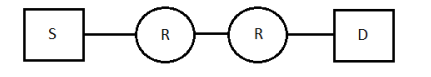
\includegraphics[width=\columnwidth]{figs/q14.png}
        \label{fig:placeholder}
    \end{figure}
    \begin{enumerate}
        \item Network layer – 4 times and Data link layer – 4 times 
        \item Network layer – 4 times and Data link layer – 3 times 
        \item Network layer – 4 times and Data link layer – 6 times 
        \item Network layer – 2 times and Data link layer – 6 times 
    \end{enumerate}

    \hfill (GATE CS 2013)

    \item An index is clustered, if
    \begin{enumerate}
        \item it is on a set of fields that form a candidate key
        \item it is on a set of fields that include the primary key
        \item the data records of the file are organized in the same order as the data entries of the index
        \item the data records of the file are organized not in the same order as the data entries of the index.
    \end{enumerate}

    \hfill (GATE CS 2013)

    \item Three concurrent processes \textit{X, Y, and }Z execute three different code segments that access and update certain shared variables. Process \textit{X} executes the P operation (i.e., \textit{wait}) on semaphores \textit{a, b} and \textit{c}; process \textit{Y} executes the \textit{P} operation on semaphores \textit{b, c and d}; process \textit{Z} executes the \textit{P} operation on semaphores \textit{c, d, and a} before entering the respective code segments. After completing the execution of its code segment, each process invokes the V operation (i.e., \textit{signal}) on its three semaphores. All semaphores are binary semaphores initialized to one. Which one of the following represents a deadlock-free order of invoking the P operations by the processes? 
    \begin{enumerate}
        \item $X: P(a)P(b)P(c) Y: P(b)P(c)P(d) Z: P(c)P(d)P(a) $
        \item $X: P(b)P(a)P(c) Y: P(b)P(c)P(d) Z: P(a)P(c)P(d)$
        \item $X: P(b)P(a)P(c) Y: P(c)P(b)P(d) Z: P(a)P(c)P(d)$
        \item $X: P(a)P(b)P(c) Y: P(c)P(b)P(d) Z: P(c)P(d)P(a) $
    \end{enumerate}

    \hfill (GATE CS 2013)
    
    \item Which of the following statements is/are \textbf{FALSE}? 
    \begin{enumerate}[label=\arabic*.]
        \item For every non-deterministic Turing machine, there exists an equivalent deterministic Turing machine.
        \item Turing recognizable languages are closed under union and complementation.
        \item Turing decidable languages are closed under intersection and complementation.
        \item Turing recognizable languages are closed under union and intersection. 
    \end{enumerate}
    \begin{enumerate}
        \begin{multicols}{4}
            \item 1 and 4 only
            \item 1 and 3 only
            \item 2 only
            \item 3 only
        \end{multicols}
    \end{enumerate}

    

    \hfill (GATE CS 2013)
    
    \item Which of the following statements is/are \textbf{TRUE}? 
    \begin{enumerate}[label=\arabic*.]
        \item The problem of determining whether there exists a cycle in an undirected graph is in P. 
        \item The problem of determining whether there exists a cycle in an undirected graph is in NP. 
        \item If a problem A is NP-Complete, there exists a non-deterministic polynomial time algorithm to solve A
    \end{enumerate}
    \begin{enumerate}
        \begin{multicols}{4}
            \item 1 ,2 and 3 only
            \item 1 and 2 only
            \item 2 and 3 only
            \item 1 and 3 only
        \end{multicols}
    \end{enumerate}

    \hfill (GATE CS 2013)

    \item What is the time complexity of Bellman-Ford single-source shortest path algorithm on a complete graph of \textit{n} vertices? 
    \begin{enumerate}
        \begin{multicols}{4}
            \item $\Theta(n^2)$
            \item $\Theta(n^2\log n)$
            \item $\Theta(n^3)$
            \item $\Theta(n^3 \log n)$
        \end{multicols}
    \end{enumerate}

    \hfill (GATE CS 2013)

    \item In a k-way set associative cache, the cache is divided into v sets, each of which consists of k lines. The lines of a set are placed in sequence one after another. The lines in set s are sequenced before the lines in set (s+1). The main memory blocks are numbered 0 onwards. The main memory block numbered j must be mapped to any one of the cache lines from
    \begin{enumerate}
        \begin{multicols}{2}
            \item (j mod v) * k to (j mod v) * k + (k-1)
            \item (j mod v) to (j mod v) + (k-1)
            \item (j mod k) to (j mod k) + (v-1)
            \item (j mod k) * v to (j mod k) * v + (v-1)
        \end{multicols}
    \end{enumerate}

    \hfill (GATE CS 2013)

    \item Which one of the following expressions does \textbf{NOT} represent exclusive NOR of x and y?
    \begin{enumerate}
        \begin{multicols}{2}
            \item $xy + x' y'$
            \item $x\bigoplus y'$
            \item $x'\bigoplus y$
            \item $x'\bigoplus y'$
        \end{multicols}
    \end{enumerate}

    \hfill (GATE CS 2013)
    
    \item Which one of the following functions is continuous at x = 3? 
    \begin{enumerate} 
    
    \item
    \[
    f(x) =
    \begin{cases} 
    2, & \text{if } x = 3,\\ 
    x - 1, & \text{if } x > 3,\\ 
    \dfrac{x+3}{3}, & \text{if } x < 3 
    \end{cases}
    \]
     
    \item  
    \[
    f(x) = 
    \begin{cases} 
    4, & \text{if } x = 3,\\ 
    8 - x, & \text{if } x \neq 3
    \end{cases}
    \]
    
    \item  
    \[
    f(x) = 
    \begin{cases} 
    x + 3, & \text{if } x \leq 3,\\ 
    x - 4, & \text{if } x > 3
    \end{cases}
    \]
     
    \item 
    \[
    f(x) =
    \begin{cases} 
    \dfrac{1}{x^3 - 27}, & \text{if } x \neq 3
    \end{cases}
    \]
     
\end{enumerate}

    

    \hfill (GATE CS 2013)
    
    \item Function f is known at the following points:\\
    \begin{tabular}{|c|c|c|c|c|c|c|c|c|c|c|c|}
    \hline
        x & 0 & 0.3 & 0.6 & 0.9 & 1.2 & 1.5 & 1.8 & 2.1 & 2.4 & 2.7 & 3.0  \\
        \hline
        $f(x)$ & 0 & 0.09 & 0.36 & 0.81 & 1.44 & 2.25 & 3.24 & 4.41 & 5.76 & 7.29 & 9.00 \\
        \hline
    \end{tabular}\\
    The value of $\int_{0}^{3} f(x)dx$computed using the trapezoidal rule is 
    \begin{enumerate}
        \begin{multicols}{4}
            \item 8.983
            \item 9.003
            \item 9.017
            \item 9.045
        \end{multicols}
    \end{enumerate}

    \hfill (GATE CS 2013)
    
    \item Consider an undirected random graph of eight vertices. The probability that there is an edge between a pair of vertices is 1/2. What is the expected number of unordered cycles of length three?
    \begin{enumerate}
        \begin{multicols}{4}
            \item 1/8
            \item 1 
            \item 7
            \item 8
        \end{multicols}
    \end{enumerate}

    \hfill (GATE CS 2013)

    \item Which of the following statements is/are TRUE for undirected graphs? 
    
    \begin{enumerate}[label=\Alph*., start=16]
        \item Number of odd degree vertices is even.
        \item Sum of degrees of all vertices is even.
    \end{enumerate}
    
    \begin{enumerate}
    \begin{multicols}{4}
        \item P only
        \item Q only
        \item Both P and Q
        \item Neither P and Q
    \end{multicols}
    \end{enumerate}
    \hfill (GATE CS 2013)

     \large\textbf{Q.26 to Q.55 carry two marks each.}\\
     \item The line graph L(G) of a simple graph G is defined as follows: 
     \begin{itemize}
         \item There is exactly one vertex v(e) in L(G) for each edge e in G. 
         \item For any two edges e and e' in \textit{G, L(G)} has an edge between \textit{v(e) and v(e')}, if and only if e and e' are incident with the same vertex in G. 
     \end{itemize}
     Which of the following statements is/are \textbf{TRUE}?
     \begin{enumerate}[label=(\Alph*), start=16]
         \item The line graph of a cycle is a cycle
         \item The line graph of a clique is a clique. 
         \item  The line graph of a planar graph is planar.
         \item The line graph of a tree is a tree.
     \end{enumerate}
     \begin{enumerate}
         \begin{multicols}{4}
             \item P only
             \item P and R only
             \item R only 
             \item P, Q and S only
         \end{multicols}
     \end{enumerate}

     \hfill (GATE CS 2013)

     \item What is the logical translation of the following statement? 
     \begin{center}
         “None of my friends are perfect.”
     \end{center}
     \begin{enumerate}
         \begin{multicols}{2}
             \item $\exists x (F (x)\land \neg P(x)) $
             \item $\exists x (\neg F (x)\land P(x))$
             \item $ \exists x (\neg F (x)\land \neg P(x)) $
             \item $\exists x (F (x)\land P(x)) $
         \end{multicols}
     \end{enumerate}

     \hfill (GATE CS 2013)
     
     \item Consider the following sequence of micro-operations\\
     
    $MBR \leftarrow PC\\
    MAR \leftarrow X\\
    PC \leftarrow Y\\
    Memory \leftarrow MBR $\\
     
     Which one of the following is a possible operation performed by this sequence? 
     \begin{enumerate}
         \begin{multicols}{2}
             \item  Instruction fetch 
             \item Operand fetch
             \item Conditional branch
             \item Initiation of interrupt service 
         \end{multicols}
     \end{enumerate}

     \hfill (GATE CS 2013)

     \item Consider a hard disk with 16 recording surfaces (0-15) having 16384 cylinders (0-16383) and each cylinder contains 64 sectors (0-63). Data storage capacity in each sector is 512 bytes. Data are organized cylinder-wise and the addressing format is <cylinder no., surface no., sector no.>. A file of size 42797 KB is stored in the disk and the starting disk location of the file is <1200, 9, 40>. What is the cylinder number of the last sector of the file, if it is stored in a contiguous manner? 
     \begin{enumerate}
         \begin{multicols}{4}
             \item 1281
             \item 1282
             \item 1283
             \item 1284
         \end{multicols}
     \end{enumerate}

     \hfill (GATE CS 2013)

     \item The number of elements that can be sorted in $\Theta(\log n)$ time using heap sort is
     \begin{enumerate}
         \begin{multicols}{4}
             \item $\Theta(1)$
             \item $\Theta(\sqrt{\log n})$
             \item $\Theta \frac{\log n}{\log\log n}$
             \item $\Theta(\log n)$
         \end{multicols}
     \end{enumerate}

\hfill (GATE CS 2013)

     \item Consider the following function:
     \begin{lstlisting}
    int unknown(int n){
        int i, j, k=0;
        for (i=n/2; i<=n; i++)
            for (j=2; j<=n; j=j*2)
                k = k + n/2;
        return (k);
    } 
    \end{lstlisting}
     The return value of the function is
     \begin{enumerate}
         \begin{multicols}{4}
            \item $\Theta(n^2)$
            \item $\Theta(n^2\log n)$
            \item $\Theta(n^3)$
            \item $\Theta(n^3 \log n)$
         \end{multicols}
     \end{enumerate}
     \hfill (GATE CS 2013)

     \item Consider the following languages. 
     \begin{center}
         $L_1 =$ \lcbrak{} $0^p1^q0^r|p,q,r \geq 0 $\rcbrak{}
         $L_2 =$ \lcbrak{} $0^p1^q0^r|p,q,r \geq 0, p\neq r $\rcbrak{}
     \end{center}
     Which one of the following statements is \textbf{FALSE}? 
     \begin{enumerate}
         \begin{multicols}{4}
             \item L2 is context-free
             \item $L1\bigcap L2$ is context-free. 
             \item Complement of L2 is recursive
             \item Complement of L1 is context-free but not regular
         \end{multicols}
     \end{enumerate}
     \hfill (GATE CS 2013)

     \item Consider the DFA A given below. 
     \begin{figure}[H]
         \centering
         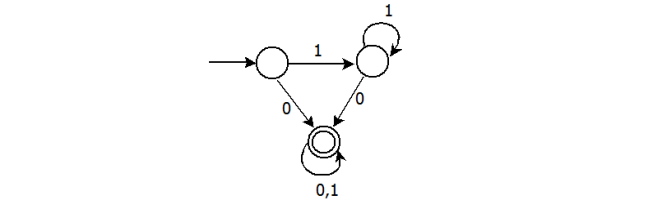
\includegraphics[width=\columnwidth]{figs/q33.png}
         \label{fig:placeholder}
     \end{figure}
     Which of the following are \textbf{FALSE}? 
     \begin{enumerate}[label=\arabic*.]
         \item Complement of L(A) is context-free.
         \item $L(A) = L((11*0+0)(0 + 1)*0*1*) $
         \item For the language accepted by A, A is the minimal DFA.
         \item A accepts all strings over {0, 1} of length at least 2.
     \end{enumerate}
     \begin{enumerate}
         \begin{multicols}{2}
             \item 1 and 3 only
             \item 2 and 4 only
             \item 2 and 3 only
             \item 3 and 4 only
         \end{multicols}
     \end{enumerate}

     \hfill (GATE CS 2013)

     \item A shared variable x, initialized to zero, is operated on by four concurrent processes W, X, Y, Z as follows. Each of the processes W and X reads x from memory, increments by one, stores it to memory, and then terminates. Each of the processes Y and Z reads x from memory, decrements by two, stores it to memory, and then terminates. Each process before reading x invokes the P operation (i.e., wait) on a counting semaphore S and invokes the V operation (i.e., signal) on the semaphore S after storing x to memory. Semaphore S is initialized to two. What is the maximum possible value of x after all processes complete execution? 
     \begin{enumerate}
         \begin{multicols}{4}
             \item -2
             \item -1
             \item 1
             \item 2
         \end{multicols}
     \end{enumerate}
\hfill (GATE CS 2013)
     \item  Consider the following relational schema. 
     
    \begin{center}
    \begin{tabular}{l}
    Students(\underline{rollno: integer}, sname: string) \\
    Courses(\underline{courseno: integer}, cname: string) \\
    Registration(\underline{rollno: integer}, \underline{courseno: integer}, percent: real)
    \end{tabular}
    \end{center}
     Which of the following queries are equivalent to this query in English? \\ “Find the distinct names of all students who score more than 90\% in the course numbered 107”
     \begin{enumerate}[label=(\Roman*)]
         \item SELECT DISTINCT S.sname\\ FROM Students as S, Registration as R \\ WHERE R.rollno=S.rollno AND R.courseno=107 AND R.percent >90 
         \item $\Pi_{sname} (\sigma_{courseno=107 \land percent} > 90 (Registration \bowtie Students)) $
         \item $\{T | \exists S \epsilon Students, \exists R \epsilon Registration ( S.rollno=R.rollno \land R.courseno=107 \land R.percent>90 \land T.sname=S.sname)\}$
         \item $\{<SN> | \exists S_R \exists R_P ( <SR, SN> \epsilon Students \land <S_R, 107, R_P> \epsilon Registration \land R_P>90)\}$ 
     \end{enumerate}
     \begin{enumerate}
         \begin{multicols}{2}
             \item I, II, III and IV
             \item I, II and III only 
             \item I, II and IV only
             \item II, III and IV only 
         \end{multicols}
     \end{enumerate}

     \hfill (GATE CS 2013)

     \item Determine the maximum length of the cable (in km) for transmitting data at a rate of 500 Mbps in an Ethernet LAN with frames of size 10,000 bits. Assume the signal speed in the cable to be 2,00,000 km/s. 
     \begin{enumerate}
         \begin{multicols}{4}
             \item 1
             \item 2
             \item 2.5
             \item 5
         \end{multicols}
     \end{enumerate}

     \hfill (GATE CS 2013)

     \item In an IPv4 datagram, the M bit is 0, the value of HLEN is 10, the value of total length is 400 and the fragment offset value is 300. The position of the datagram, the sequence numbers of the first and the last bytes of the payload, respectively are
     \begin{enumerate}
         \begin{multicols}{2}
             \item Last fragment, 2400 and 2789 
             \item First fragment, 2400 and 2759 
             \item Last fragment, 2400 and 2759 
             \item Middle fragment, 300 and 689 

         \end{multicols}
     \end{enumerate}

     \hfill (GATE CS 2013)
     \item The following figure represents access graphs of two modules M1 and M2. The filled circles represent methods and the unfilled circles represent attributes. If method m is moved to module M2 keeping the attributes where they are, what can we say about the average cohesion and coupling between modules in the system of two modules?
     \begin{figure}
         \centering
         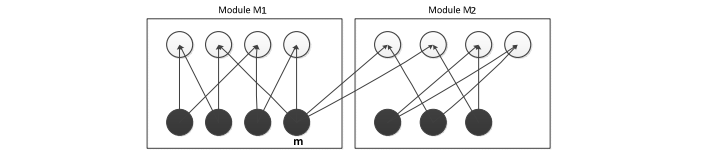
\includegraphics[width=\columnwidth]{figs/q38.png}
         \label{fig:placeholder}
     \end{figure}
     \begin{enumerate}
         \begin{multicols}{2}
             \item There is no change. 
             \item Average cohesion goes up but coupling is reduced. 
             \item Average cohesion goes down and coupling also reduces.
             \item Average cohesion and coupling increase.
         \end{multicols}
     \end{enumerate}

     \hfill (GATE CS 2013)

     \item A certain computation generates two arrays a and b such that a[i]=f(i)for $0 \leq i < n$ and b[i] = g (a[i] )for $0 \leq i < n$. Suppose this computation is decomposed into two concurrent processes X and Y such that X computes the array a and Y computes the array b. The processes employ two binary semaphores R and S, both initialized to zero. The array a is shared by the two processes. The structures of the processes are shown below.
     \begin{enumerate}[label=]
         \begin{multicols}{2}
            \item Process X:\\
            \begin{lstlisting}
            private i;
            for (i=0; i<n; i++) {
            a[i] = f(i);
            ExitX(R, S);
            }
            \end{lstlisting}
            \item Process Y:\\
            \begin{lstlisting}
            private i;
            for (i=0; i<n; i++) {
            EntryY(R, S);
            b[i] = g(a[i]);
            }
            \end{lstlisting}
         \end{multicols}
     \end{enumerate}
     Which one of the following represents the CORRECT implementations of \texttt{ExitX and EntryY} ?
            \begin{minipage}{0.45\textwidth}
            \textbf{(A)}
            \begin{lstlisting}
            ExitX(R, S) {
                P(R);
                V(S);
            }
            EntryY(R, S) {
                P(S);
                V(R);
            }
            \end{lstlisting}
            
            \medskip
            \textbf{(C)}
            \begin{lstlisting}
            ExitX(R, S) {
                P(S);
                V(R);
            }
            EntryY(R, S) {
                V(S);
                P(R);
            }
            \end{lstlisting}
            \end{minipage}
            \hfill
            \begin{minipage}{0.45\textwidth}
            \textbf{(B)}
            \begin{lstlisting}
            ExitX(R, S) {
                V(R);
                V(S);
            }
            EntryY(R, S) {
                P(R);
                P(S);
            }
            \end{lstlisting}
            
            \medskip
            \textbf{(D)}
            \begin{lstlisting}
            ExitX(R, S) {
                V(R);
                P(S);
            }
            EntryY(R, S) {
                V(S);
                P(R);
            }
            \end{lstlisting}
            \end{minipage}

            \hfill (GATE CS 2013)
    \item Consider the following two sets of LR(1) items of an LR(1) grammar. \\
    \begin{tabular}{cc}
        X → c.X, c/d & X → c.X, \$  \\
        X → .cX, c/d & X → .cX, \$ \\
        X → .d, c/d  & X → .d, \$ 

    \end{tabular}\\
    Which of the following statements related to merging of the two sets in the corresponding LALR parser is/are FALSE?
    \begin{enumerate}[label=\arabic*]
        \item Cannot be merged since look aheads are different
        \item Can be merged but will result in S-R conflict. 
        \item Can be merged but will result in R-R conflict. 
        \item Cannot be merged since goto on c will lead to two different sets.
    \end{enumerate}
    \begin{enumerate}
    \begin{multicols}{2}
        \item 1 only
        \item 2 only
        \item 1 and 4 only
        \item 1, 2,3 and 4 only
    \end{multicols}
    \end{enumerate}
    \hfill (GATE CS 2013)

     \item Which of the following is/are undecidable? 
     \begin{enumerate}
         \item $G is a CFG. Is L(G) = \Phi?  $
         \item $G is a CFG. Is L(G) = \sum*?$
         \item M is a Turing machine. Is L(M) regular? 
         \item A is a DFA and N is an NFA. Is L(A) = L(N)? 
     \end{enumerate}
     \begin{enumerate}
         \begin{multicols}{2}
             \item 3 only
             \item 3 and 4 only
             \item 1, 2 and 3 only
             \item 2 and 3 only
         \end{multicols}
     \end{enumerate}
     \hfill (GATE CS 2013)

     \item What is the return value of f(p,p), if the value of p is initialized to 5 before the call? Note that the first parameter is passed by reference, whereas the second parameter is passed by value. 
     \begin{lstlisting}
        int f (int &x, int c) {
        c = c - 1;
        if (c==0) return 1;
        x = x + 1;
        return f(x,c) * x;
        }

     \end{lstlisting}
     \begin{enumerate}
         \begin{multicols}{4}
             \item 3024
             \item 6561
             \item 55440
             \item 161051
         \end{multicols}
     \end{enumerate}
     \hfill (GATE CS 2013)

     \item The preorder traversal sequence of a binary search tree is 30, 20, 10, 15, 25, 23, 39, 35, 42. Which one of the following is the postorder traversal sequence of the same tree? 
     \begin{enumerate}
         \begin{multicols}{2}
             \item 10, 20, 15, 23, 25, 35, 42, 39, 30
             \item 15, 10, 25, 23, 20, 42, 35, 39, 30
             \item 15, 20, 10, 23, 25, 42, 35, 39, 30 
             \item 15, 10, 23, 25, 20, 35, 42, 39, 30 
         \end{multicols}
     \end{enumerate}
     \hfill (GATE CS 2013)

     \item Consider the following operation along with Enqueue and Dequeue operations on queues, where k is a global parameter.
     \begin{lstlisting}
         MultiDequeue(Q){
         m = k
         while (Q is not empty) and (m > 0) {
         Dequeue(Q)
         m = m - 1
         }
         }
     \end{lstlisting}
     What is the worst case time complexity of a sequence of n queue operations on an initially empty queue?
     \begin{enumerate}
         \begin{multicols}{4}
             \item $\Theta(n)$
             \item $\Theta(n+k)$
             \item $\Theta(nk)$
             \item $\Theta(n^2)$
         \end{multicols}
     \end{enumerate}
     \hfill (GATE CS 2013)

     \item Consider an instruction pipeline with five stages without any branch prediction: Fetch Instruction (FI), Decode Instruction (DI), Fetch Operand (FO), Execute Instruction (EI) and Write Operand (WO). The stage delays for FI, DI, FO, EI and WO are 5 ns, 7 ns, 10 ns, 8 ns and 6 ns, respectively. There are intermediate storage buffers after each stage and the delay of each buffer is 1 ns. A program consisting of 12 instructions I1, I2, I3, …, I12 is executed in this pipelined processor. Instruction I4 is the only branch instruction and its branch target is I9. If the branch is taken during the execution of this program, the time (in ns) needed to complete the program is
     \begin{enumerate}
         \begin{multicols}{4}
             \item 132
             \item 165
             \item 176
             \item 328
         \end{multicols}
     \end{enumerate}
     \hfill (GATE CS 2013)
     \item A RAM chip has a capacity of 1024 words of 8 bits each (1K × 8). The number of 2 × 4 decoders with enable line needed to construct a 16K × 16 RAM from 1K × 8 RAM is 
     \begin{enumerate}
         \begin{multicols}{4}
             \item 4
             \item 5
             \item 6
             \item 7
         \end{multicols}
     \end{enumerate}
     \hfill (GATE CS 2013)

     \item Which one of the following is NOT logically equivalent to $\sigma \exists x (\forall y (\alpha)\land \forall z(\beta ))$?
     \begin{enumerate}
         \begin{multicols}{2}
             \item $\forall x (\exists z(\neg \beta )\rightarrow \forall y (\alpha)) $
             \item $\forall x (\forall  z(\beta ) \rightarrow\exists y (\neg \alpha))$
             \item $\forall x (\forall  y (\alpha)\rightarrow \exists z(\neg \beta )) $
             \item $\forall x (\exists y (\neg \alpha)\rightarrow \exists z(\neg \beta ))$
         \end{multicols}
     \end{enumerate}
     \hfill (GATE CS 2013)

    \textbf{Common Data Questions}\\
    \textbf{Common Data for Questions 48 and 49:}\\
    The following code segment is executed on a processor which allows only register operands in its instructions. Each instruction can have atmost two source operands and one destination operand. Assume that all variables are dead after this code segment.
    \begin{lstlisting}
        c = a + b;
        d = c * a;
        e = c + a;
        x = c * c;
        if (x > a) {
            y = a * a;
        }
        else {
            d = d * d;
            e = e * e;
        } 

    \end{lstlisting}
    \item Suppose the instruction set architecture of the processor has only two registers. The only allowed compiler optimization is code motion, which moves statements from one place to another while preserving correctness. What is the minimum number of spills to memory in the compiled code?
    \begin{enumerate}
         \begin{multicols}{4}
             \item 0
             \item 1
             \item 2
             \item 3
         \end{multicols}
     \end{enumerate}
     \hfill (GATE CS 2013)

     \item What is the minimum number of registers needed in the instruction set architecture of the processor to compile this code segment without any spill to memory? Do not apply any optimization other than optimizing register allocation.
     \begin{enumerate}
         \begin{multicols}{4}
             \item 3
             \item 4
             \item 5
             \item 6
         \end{multicols}
     \end{enumerate}
     \hfill (GATE CS 2013)

     \textbf{Common Data for Questions 50 and 51:}\\
     The procedure given below is required to find and replace certain characters inside an input character string supplied in array A. The characters to be replaced are supplied in array oldc, while their respective replacement characters are supplied in array newc. Array A has a fixed length of five characters, while arrays oldc and newc contain three characters each. However, the procedure is flawed.
     \begin{lstlisting}
         void find_and_replace (char *A, char *oldc, char *newc) {
                for (int i=0; i<5; i++)
                   for (int j=0; j<3; j++)
                         if (A[i] == oldc[j]) A[i] = newc[j];
        } 

     \end{lstlisting}
     The procedure is tested with the following four test cases. 
     \begin{enumerate}
         \begin{multicols}{2}
             \item \texttt{oldc = “abc”, newc = “dab”}
             \item \texttt{oldc = “cde”, newc = “bcd”}
             \item \texttt{oldc = “bca”, newc = “cda” }
             \item \texttt{oldc = “abc”, newc = “bac”}
         \end{multicols}
     \end{enumerate}
     \hfill (GATE CS 2013)

     \item The tester now tests the program on all input strings of length five consisting of characters ‘a’, ‘b’, ‘c’, ‘d’ and ‘e’ with duplicates allowed. If the tester carries out this testing with the four test cases given above, how many test cases will be able to capture the flaw?
     \begin{enumerate}
         \begin{multicols}{4}
             \item Only one
             \item Only two
             \item Only three 
             \item All four
         \end{multicols}
     \end{enumerate}
     \hfill (GATE CS 2013)

     \item If array A is made to hold the string \texttt{“abcde”}, which of the above four test cases will be successful in exposing the flaw in this procedure? 
     \begin{enumerate}
         \begin{multicols}{4}
             \item None
             \item 2 only 
             \item 3 and 4 only 
             \item 4 only
         \end{multicols}
     \end{enumerate}
     \hfill (GATE CS 2013)

    \textbf{Linked Answer Questions}\\
    \textbf{Statement for Linked Answer Questions 52 and 53: }\\
    A computer uses 46-bit virtual address, 32-bit physical address, and a three-level paged page table organization. The page table base register stores the base address of the first-level table (T1), which occupies exactly one page. Each entry of T1 stores the base address of a page of the second-level table (T2). Each entry of T2 stores the base address of a page of the third-level table (T3). Each entry of T3 stores a page table entry (PTE). The PTE is 32 bits in size. The processor used in the computer has a 1 MB 16-way set associative virtually indexed physically tagged cache. The cache block size is 64 bytes.
    \item What is the size of a page in KB in this computer? 
    \begin{enumerate}
         \begin{multicols}{4}
             \item 2
             \item 4
             \item 8
             \item 16
         \end{multicols}
     \end{enumerate}
     \hfill (GATE CS 2013)

     \item What is the minimum number of page colours needed to guarantee that no two synonyms map to different sets in the processor cache of this computer? 
    \begin{enumerate}
         \begin{multicols}{4}
             \item 2
             \item 4
             \item 8
             \item 16
         \end{multicols}
     \end{enumerate}
     \hfill (GATE CS 2013)

     \textbf{Statement for Linked Answer Questions 54 and 55: }\\
     Relation R has eight attributes ABCDEFGH. Fields of R contain only atomic values. F=${CH\rightarrow G, A\rightarrow BC, B\rightarrow CFH, E\rightarrow A, F\rightarrow EG}$ is a set of functional dependencies (FDs) so that F + is exactly the set of FDs that hold for R. 
     \item How many candidate keys does the relation R have?
     \begin{enumerate}
         \begin{multicols}{4}
             \item 3
             \item 4
             \item 5
             \item 6
         \end{multicols}
     \end{enumerate}
     \hfill (GATE CS 2013)

     \item The relation R is 
     \begin{enumerate}
         \begin{multicols}{2}
             \item in 1NF, but not in 2NF
             \item in 2NF, but not in 3NF.
             \item in 3NF, but not in BCNF. 
             \item in BCNF. 
         \end{multicols}
     \end{enumerate}
     \hfill (GATE CS 2013)

     \newpage

     \textbf{General Aptitude (GA) Questions}\\
     \textbf{Q.56 to Q.60 carry one mark each.}\\


     \item Which one of the following options is the closest in meaning to the word given below? \\
     \textbf{Nadir }
     \begin{enumerate}
         \begin{multicols}{4}
             \item Highest
             \item Lowest
             \item Medium
             \item Integration
         \end{multicols}
     \end{enumerate}
     \hfill (GATE CS 2013)

     \item Complete the sentence: \\ Universalism is to particularism as diffuseness is to \underline{\hspace{2cm}}.
     \begin{enumerate}
         \begin{multicols}{4}
             \item specificity
             \item neutrality
             \item generality
             \item adaptation
         \end{multicols}
     \end{enumerate}
     \hfill (GATE CS 2013)

     \item What will be the maximum sum of 44, 42, 40, ...... ?
     \begin{enumerate}
         \begin{multicols}{4}
             \item 502
             \item 504
             \item 506
             \item 500
         \end{multicols}
     \end{enumerate}
     \hfill (GATE CS 2013)

     \item Were you a bird, you \underline{\hspace{2cm}}. in the sky. 
     \begin{enumerate}
         \begin{multicols}{4}
             \item would fly
             \item shall fly
             \item should fly 
             \item shall have flown
         \end{multicols}
     \end{enumerate}
     \hfill (GATE CS 2013)
     
     \item Choose the grammatically \textbf{INCORRECT} sentence: 
     \begin{enumerate}
         \begin{multicols}{2}
             \item He is of Asian origin
             \item They belonged to Africa.
             \item She is an European. 
             \item They migrated from India to Australia.
         \end{multicols}
     \end{enumerate}
     \hfill (GATE CS 2013)

     \textbf{Q.61 to Q.65 carry two marks each. }\\

     \item Find the sum of the expression
     $\frac{1}{\sqrt{1}+\sqrt2}+\frac{1}{\sqrt{2}+\sqrt3}+\frac{1}{\sqrt{3}+\sqrt4}+..........\frac{1}{\sqrt{80}+\sqrt81}$
     \begin{enumerate}
         \begin{multicols}{2}
             \item 7
             \item 8
             \item 9
             \item 10
         \end{multicols}
     \end{enumerate}

     \hfill (GATE CS 2013)

     \item Out of all the 2-digit integers between 1 and 100, a 2-digit number has to be selected at random. What is the probability that the selected number is not divisible by 7?
     \begin{enumerate}
         \begin{multicols}{2}
             \item 13/90 
             \item 12/90 
             \item 78/90
             \item 77/90 
         \end{multicols}
     \end{enumerate}

     \hfill (GATE CS 2013)

     \item After several defeats in wars, Robert Bruce went in exile and wanted to commit suicide. Just before committing suicide, he came across a spider attempting tirelessly to have its net. Time and again, the spider failed but that did not deter it to refrain from making attempts. Such attempts by the spider made Bruce curious. Thus, Bruce started observing the near-impossible goal of the spider to have the net. Ultimately, the spider succeeded in having its net despite several failures. Such act of the spider encouraged Bruce not to commit suicide. And then, Bruce went back again and won many a battle, and the rest is history.\\ Which one of the following assertions is best supported by the above information? 
     \begin{enumerate}
         \begin{multicols}{2}
             \item Failure is the pillar of success. 
             \item Honesty is the best policy.  
             \item Life begins and ends with adventures. 
             \item No adversity justifies giving up hope.
         \end{multicols}
     \end{enumerate}

     \hfill (GATE CS 2013)

     \item A tourist covers half of his journey by train at 60 km/h, half of the remainder by bus at 30 km/h and the rest by cycle at 10 km/h. The average speed of the tourist in km/h during his entire journey is
     \begin{enumerate}
         \begin{multicols}{4}
             \item 36
             \item 30  
             \item 24
             \item 18
         \end{multicols}
     \end{enumerate}

     \hfill (GATE CS 2013)

     \item The current erection cost of a structure is Rs. 13,200. If the labour wages per day increase by 1/5 of the current wages and the working hours decrease by 1/24 of the current period, then the new cost of erection in Rs. is 
     \begin{enumerate}
         \begin{multicols}{4}
             \item 16,500
             \item 15,180  
             \item 11,000 
             \item 10,120 
         \end{multicols}
     \end{enumerate}
\hfill (GATE CS 2013)

\begin{center}
    \Large END OF THE QUESTION PAPER
\end{center}
    
 \end{enumerate}
\end{document}
